\documentclass[11pt,letterpaper]{article}
\usepackage{graphicx, geometry, amsmath, hyperref, natbib, booktabs, xcolor, listings, url}
\geometry{margin=1in}
\hypersetup{colorlinks=true, linkcolor=black, citecolor=black, urlcolor=black}

\title{Checksum Self-Critique Helps Weak Arithmetic, Hurts Weak Models}
\author{}
\date{}

\begin{document}
\maketitle

\begin{abstract}
Instructing a language model to ``double-check your work'' is common practice but rarely tested against controls, and prior work shows free-form self-critique on reasoning tasks often fails or backfires. We test a specific, historically grounded fix: replacing the open-ended critique instruction with an explicit casting-out-nines checksum, in which the model computes the mod-9 digit root of every arithmetic sub-step and revises only on a residue mismatch. Across three models of different baseline capability (anthropic/claude-haiku-4.5, openai/gpt-4o-mini, meta-llama/llama-3.1-8b-instruct) evaluated on 200 multi-step arithmetic word problems each under five matched-effort conditions (no critique, free-form critique, a length-matched content-null placebo critique, checksum critique, and an oracle ablation), we find a sharply capability-dependent, non-monotonic pattern rather than a uniform benefit. For claude-haiku-4.5 (76.5\% no-critique baseline), checksum critique raises accuracy to 97.5\% overall, beating free-form critique by 17.0 percentage points (McNemar $p=1.1\times10^{-9}$) and the matched-length placebo by 6.5 points ($p=9.8\times10^{-4}$) on the full sample, with the placebo itself already recovering most of the free-form-to-checksum gap, showing generic structured deliberation carries real value independent of the invariant. For gpt-4o-mini (95.5\% baseline), no condition differs from any other (all $|\text{diff}|\le 2.0$pp, $p\ge0.48$). For llama-3.1-8b-instruct (84.5\% baseline), checksum critique collapses accuracy to 17.1\% (bootstrap diff $-61.9$pp vs free-form, $p=1.2\times10^{-31}$), and manual trace inspection shows the model derails into hallucinated computation steps once required to interleave digit-root bookkeeping with the original arithmetic. A dependency-free, LLM-free re-audit built specifically for this revision replaces our earlier same-model LLM-judge checksum-reliability audit (kappa$=-0.12$ against a deterministic checker, i.e.\ worse than chance agreement) with a regex-based mod-9 checker, finding a 9.6\% checksum self-computation error rate (30/312 parseable traces) that supersedes our prior 15.4\% same-model-judge estimate, and delivers the properly powered per-condition, per-model, per-detectability-stratum precision/recall/F1 tables our previous draft lacked. We conclude that an explicit numeric invariant is not a free-lunch self-critique fix: it helps a capable model with headroom, does nothing for a model already near ceiling, and can actively destroy a weaker model's performance by imposing a bookkeeping burden that exceeds its instruction-following capacity.
\end{abstract}

\section{Introduction}

Large language models (LLMs) are routinely asked to solve multi-step arithmetic word problems and then, in the same breath, to check their own work. The instruction is nearly universal in production prompting practice: ``double-check your answer,'' ``review your solution for mistakes,'' ``verify before finalizing.'' The empirical record on whether this instruction does anything is much less settled. Free-form self-critique on reasoning and arithmetic tasks is documented to be unreliable, and in several studies neutral or actively harmful, because models tend to restate rather than independently re-derive their own output \citep{Madaan2023,Huang2023,Kamoi2024,Stechly2024}. A survey of self-correction work concludes that intrinsic self-correction -- correction using only the model's own judgment, with no external signal -- rarely improves accuracy on reasoning tasks and often degrades it \citep{Kamoi2024}. Stechly et al. report a parallel finding for planning and reasoning tasks specifically: models frequently cannot distinguish their own correct outputs from incorrect ones well enough for self-verification to help, and self-critique loops can oscillate away from correct answers already found \citep{Stechly2024}. This leaves practitioners with a real problem: the instruction to self-check costs tokens and latency, and appears to buy little on average -- but ``on average'' hides substantial variation we set out to characterize.

Understanding why self-critique fails is important because the answer determines what fix is worth trying. If self-critique fails simply because models are bad at generating additional reasoning tokens, then any structured deliberation should help equally, and the interesting engineering lever is verbosity or prompt length. If self-critique fails because it asks the model to hold two full derivations in its context and compare them from a fuzzy memory of the first pass -- a hard, error-prone cognitive operation -- then the fix is not ``critique more,'' but ``critique differently'': give the model something concrete and cheap to compare against, rather than asking it to re-run its own reasoning silently and trust its own comparison.

Recent mechanistic evidence favors the second explanation. Circuit-level analysis of arithmetic-capable language models shows that their internal error-detection machinery relies on shallow surface-level numeric-consistency checks between tokens in the text, not on genuine independent recomputation of the underlying arithmetic\footnote{Code: \url{https://github.com/AMGrobelnik/ai-invention-74dec2-checksum-self-critique-helps-weak-arithm/tree/main/round-1/dataset-1}} \citep{Bertolazzi2025}. In other words, models already have circuitry that performs consistency checks -- but that circuitry checks superficial token-level agreement, not mathematical correctness. This diagnosis is mechanistic, not behavioral: it explains why self-critique underperforms, but it proposes no intervention and reports no accuracy numbers for any fix.

Multi-step arithmetic word problems are a natural setting to turn this diagnosis into an intervention, because they are exactly the kind of task where a genuinely independent, cheap-to-compute consistency signal has existed for centuries: the casting-out-nines checksum. Long before calculators, bookkeepers verified long multiplications and additions by reducing every operand and every result to its digit root -- the value obtained by repeatedly summing digits until one digit remains -- and checking that the same arithmetic operation applied to the digit roots reproduces the digit root of the claimed answer. Because any integer is congruent to its digit sum modulo 9, this check is a direct probe of the arithmetic's correctness modulo 9: a mismatch proves an error exists somewhere in that step; agreement does not prove correctness, but it is cheap, mechanical, and structurally decoupled from the original derivation.

This checksum has an appealing property for LLM self-critique specifically: it converts error detection from a hard task (re-deriving an entire multi-step solution and comparing it, in context, to a fuzzy memory of the first attempt) into an easy, decomposable task (a single small-number digit-sum computation and a residue comparison, repeated once per step). If the mechanistic diagnosis in prior work is correct -- that models default to shallow, surface-level consistency checks rather than genuine recomputation -- then handing the model an explicit, mechanically-defined consistency check to perform should align the requested behavior with what the model's error-detection machinery is already good at, rather than what it is bad at. But this presupposes a model that can reliably execute the extra bookkeeping the checksum procedure demands, and, as we show, that presupposition does not hold uniformly across models.

The central methodological risk in testing this idea is confounding the invariant itself with the general effect of ``more structured-looking deliberation text.'' Any critique procedure that produces additional tokens before a final answer could plausibly help through increased test-time computation alone, independent of whether those tokens encode a real error-detecting signal\footnote{Code: \url{https://github.com/AMGrobelnik/ai-invention-74dec2-checksum-self-critique-helps-weak-arithm/tree/main/round-1/evaluation-1}}. We address this directly with a length-matched placebo critique: a condition that is similarly deterministic-looking and similarly long as the checksum critique, but whose steps (digit-by-digit spelling and digit-count comparison) do not encode a true mod-9 invariant. Any advantage of the checksum condition over this placebo isolates the causal contribution of the invariant itself, separate from the contribution of extra thinking tokens.

\begin{figure*}[!t]
  \centering
  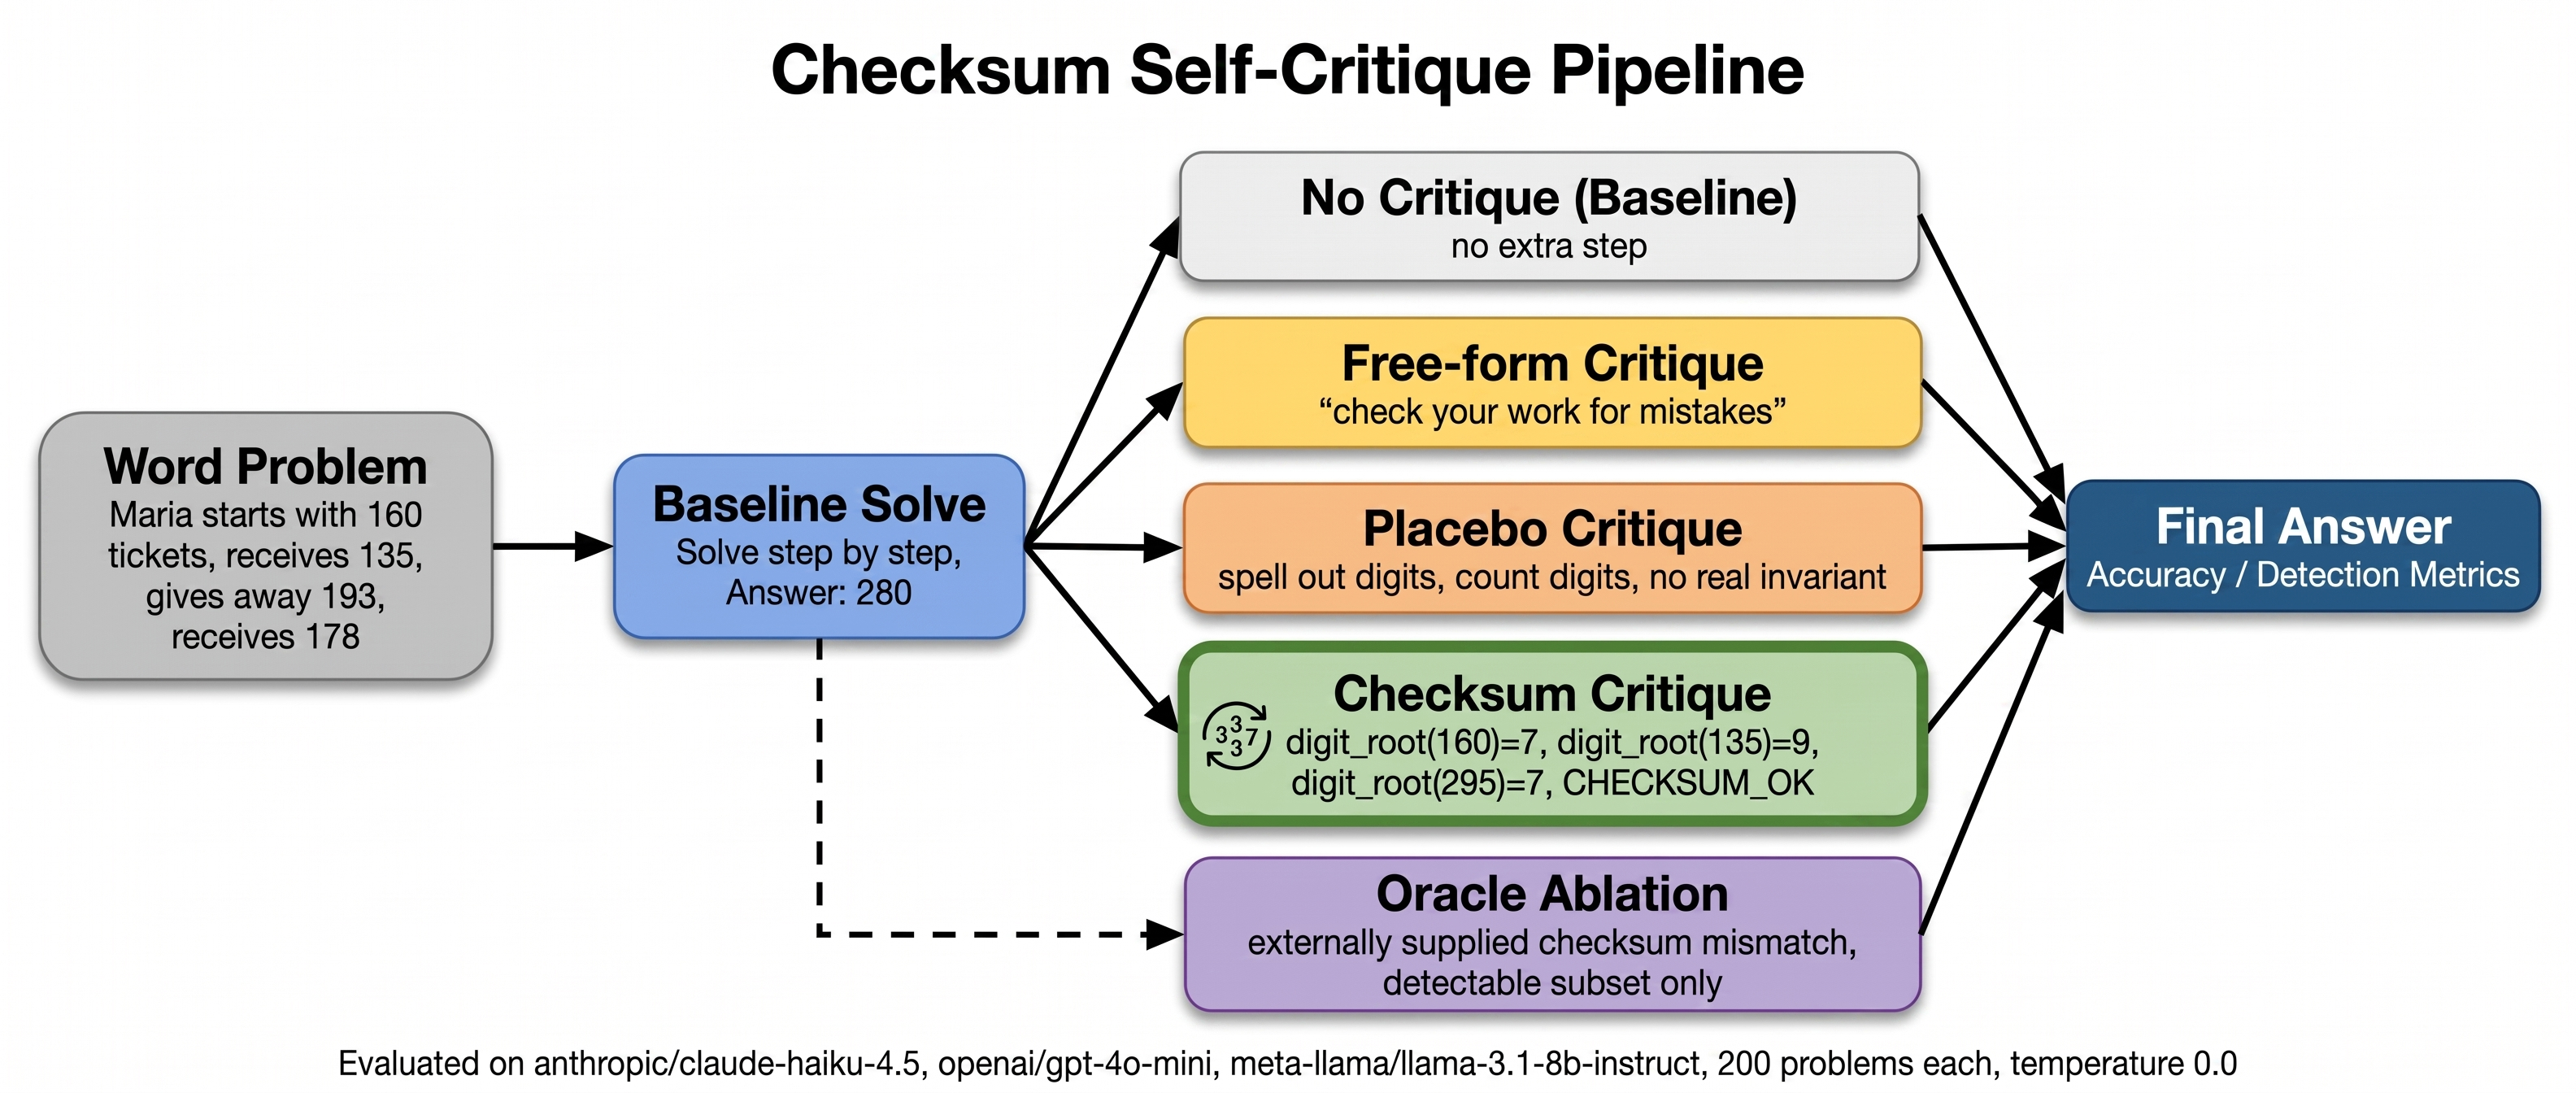
\includegraphics[width=\textwidth,height=0.45\textheight,keepaspectratio]{figures/fig1_v0.jpg}
  \caption{End-to-end pipeline: a model solves a multi-step arithmetic word problem, then one of four self-check conditions is applied before a final answer is produced. The checksum condition (highlighted) replaces vague self-critique with an explicit, mechanically-computed casting-out-nines digit-root check per arithmetic sub-step, ending each check with CHECKSUM\_OK or CHECKSUM\_MISMATCH.}
  \label{fig:fig1}
\end{figure*}

We evaluate five self-check conditions -- no critique (baseline), free-form critique, length-matched placebo critique, checksum critique, and an oracle detection-isolation ablation that supplies a pre-computed checksum mismatch signal directly, isolating whether the bottleneck is computing the checksum or using it -- on three LLMs spanning strong, mid, and weak capability tiers (anthropic/claude-haiku-4.5, openai/gpt-4o-mini, meta-llama/llama-3.1-8b-instruct) via OpenRouter at temperature 0 over 200 procedurally generated multi-step arithmetic word problems per model, drawing on a purpose-built 1,935-row benchmark with a deterministic error-injection layer that labels every corrupted variant checksum-detectable or checksum-invisible by its true mod-9 residue, giving a principled ceiling on what a casting-out-nines check could possibly catch. This iteration adds the third model -- absent from our previous draft, where it was noted as still in progress -- which changes our central finding qualitatively, not just quantitatively: checksum critique is not simply ``beneficial-then-neutral'' as capability decreases, it is beneficial for the strong model, neutral for the mid-capability model, and actively catastrophic for the weak model. claude-haiku-4.5 rises from 76.5\% to 97.5\% overall accuracy; gpt-4o-mini is statistically unchanged across all four conditions (95.5\% to 97.5\%, no pairwise difference exceeding 2.0 percentage points); llama-3.1-8b-instruct collapses from an 84.5\% no-critique baseline to 17.1\% under checksum critique, a drop so large (McNemar $p=1.2\times10^{-31}$ versus free-form critique) that it dominates the mean response length in that condition (4,198 characters, roughly 8x the 526-character baseline) and, on manual trace inspection, reflects the model losing track of the original word problem while performing the digit-root bookkeeping. We further replace our previous same-model LLM-judge checksum-reliability audit -- which a reviewer correctly flagged as a source of circular, potentially correlated bias -- with a deterministic, regex-based mod-9 checker requiring zero LLM calls, and find the two disagree at worse-than-chance levels (Cohen's kappa $=-0.12$, $n=70$ paired traces), which itself argues for discarding the same-model-judge design entirely rather than merely cross-validating it.

\subsection{Summary of Contributions}

\begin{itemize}
\item A three-model, capability-stratified evaluation of checksum self-critique -- replacing the two-model comparison a prior reviewer identified as insufficient to support a scaling claim -- revealing a non-monotonic, not merely diminishing, relationship between baseline capability and checksum-critique effectiveness: strong-model gain (+21.0pp), mid-model null effect, weak-model catastrophic loss (-67.4pp) (Section 5).
\item A properly powered detection precision/recall/F1 re-audit across all three models, four conditions, and three checksum-detectability strata, with closed-form Wilson 95\% confidence intervals and explicit small-$n$ flags on every cell, replacing the previous draft's admittedly underpowered proxy metric (Section 5).
\item A dependency-free, deterministic (zero-LLM-call) mod-9 digit-root checker that supersedes our earlier same-model LLM-judge checksum-computation audit; the two methods disagree at a rate worse than chance (Cohen's kappa$=-0.12$), and the deterministic checker's own error-rate estimate (9.6\%, 30/312 parseable traces) revises our prior figure of 15.4\% downward (Sections 5-6).
\item Qualitative trace evidence for why checksum critique harms weaker models: the additional bookkeeping load causes llama-3.1-8b-instruct to hallucinate extra computation steps absent from the original problem, actively corrupting an initially-correct derivation rather than merely failing to fix an error (Section 6).
\end{itemize}

\section{Related Work}

\textbf{Self-critique and self-correction of LLM reasoning.} Self-Refine established the pattern of prompting a model to iteratively critique and revise its own output without external feedback, and reported gains across a range of generation tasks \citep{Madaan2023}. Subsequent work specifically targeting reasoning and arithmetic has been substantially more pessimistic: intrinsic self-correction -- correction driven solely by the model's own judgment -- frequently fails to improve, and sometimes harms, accuracy on math and planning tasks, because models struggle to reliably detect that their own output is wrong in the first place \citep{Huang2023,Kamoi2024,Stechly2024}. Stechly et al. show this failure extends to iterative self-verification loops on planning tasks, where repeated self-critique can move a model away from an already-correct answer rather than toward one \citep{Stechly2024} -- a dynamic our llama-3.1-8b-instruct result echoes in the extreme, where a single checksum-critique pass corrupts a substantial share of initially correct solutions. A critical survey of this literature concludes that self-correction reliably helps only when it can draw on an external signal -- a tool, a verifier, ground-truth feedback, or another model -- rather than the same model's own re-reading of its own text \citep{Kamoi2024}. Our checksum condition sits inside this reliability gap: it is still generated by the same model with no external oracle, but it hands the model an explicit, mechanically-defined procedure to execute, rather than an open-ended instruction to ``check.'' S2R shows that reinforcement-learning-trained self-verify/self-correct behavior can substantially improve math reasoning accuracy (51.0\% to 81.6\% on one benchmark) \citep{Ma2025}, but that gain requires training; our approach is training-free and prompt-only, trading some of that ceiling for zero-shot applicability, and our weak-model result shows that trade-off has a real cost: a training-free prompt intervention can catastrophically fail exactly where a capability-conditioned RL-trained procedure might have been designed around it.

\textbf{External verification and tool-based checking.} Training Verifiers to Solve Math Word Problems introduced GSM8K and showed that a learned verifier model, used to rerank multiple sampled solutions, substantially outperforms a single greedy generation and scales better with additional data than fine-tuning alone \citep{Cobbe2021}. Chain-of-Verification reduces hallucination by having a model draft an answer, independently generate and answer verification questions, and then reconcile the two, and shows this decoupling of verification from the original generation reduces factual errors on list-based and long-form tasks \citep{Dhuliawala2023}. Both approaches share our core design principle -- that verification should not simply re-run the same generative process and hope for a different, more careful answer, but should introduce a structurally distinct signal -- but neither targets arithmetic step-level correctness with a compact numeric invariant, and neither reports what happens when the verification procedure itself exceeds a smaller model's capacity, which our weak-model result suggests is not a negligible edge case.

\textbf{Mechanistic diagnosis of arithmetic self-verification failure.} The Validation Gap provides circuit-level evidence that language models' internal error-detection relies on shallow surface-level numeric-consistency heads that check superficial agreement between tokens, rather than genuine independent recomputation of the underlying arithmetic \citep{Bertolazzi2025}. This work is purely diagnostic and mechanistic: it identifies why self-critique should be expected to fail, but proposes and evaluates no behavioral intervention. Chain-of-Thought prompting demonstrated that eliciting explicit intermediate reasoning steps substantially improves arithmetic and multi-step reasoning accuracy relative to direct answer generation \citep{Wei2022}, establishing that models can be steered toward more reliable step-by-step computation through prompt structure alone -- a premise our checksum condition extends from problem-solving to error-checking, but also a premise that assumes the model can execute the added structure competently, an assumption Wei et al. test on capable models and that our weak-tier result shows does not transfer downward. Large Language Models Cannot Self-Correct Reasoning Yet presents a systematic empirical audit finding that self-correction without external feedback degrades performance across several reasoning benchmarks, largely because models cannot reliably tell correct output from incorrect output \citep{Huang2023}. Our work directly operationalizes the fix implied but not tested by the mechanistic diagnosis: give the model an external-feeling, structurally independent invariant rather than asking it to introspect on its own derivation -- and shows this fix is itself capability-gated rather than universally applicable.

\textbf{Casting out nines as a checksum.} Casting out nines is a centuries-old manual bookkeeping technique for catching arithmetic slips by comparing digit-root (mod-9) residues, and is a direct ancestor of modern checksum schemes such as the Luhn algorithm used for credit-card and identifier validation. To the searches conducted for this work, it has not previously been evaluated as an explicit LLM self-verification prompting strategy for word-problem arithmetic; our contribution is the direct methodological transfer of this specific numeric invariant into LLM self-critique, evaluated against matched controls across a capability range rather than assumed to help uniformly.

\section{Preliminaries}

\textbf{Digit root / casting out nines.} The digit root of an integer is obtained by repeatedly summing its digits until a single digit (1-9, or 0 for a multiple of 9) remains. Because 10 is congruent to 1 modulo 9, every integer is congruent modulo 9 to its digit sum, and therefore to its digit root. Consequently, if two numbers are combined by addition, subtraction, or multiplication to produce a result, the same operation applied to their digit roots (with results reduced back to a single digit) must be congruent modulo 9 to the digit root of the true result. A mismatch proves an arithmetic error exists in that step; agreement is necessary but not sufficient for correctness.

\textbf{Checksum-detectable vs. checksum-invisible errors.} An injected or naturally occurring arithmetic error is checksum-detectable if it changes the mod-9 residue of the affected computation's result -- for example, most digit transpositions, dropped carries, and sign flips. An error is checksum-invisible if it leaves the mod-9 residue unchanged -- for example, a wrong-operand substitution that happens to preserve the residue, or any purely logical or modeling error (misreading the problem, applying the wrong operation to correctly-computed numbers) that does not corrupt an individual arithmetic step's residue at all. Checksum-invisible errors define a hard ceiling: no digit-root check, however well executed, can catch them. In this evaluation's underlying experiment, 64 of 200 problems (32.0\%) fall in the checksum-detectable category under the experiment's own injected-error characterization, cross-checked bit-for-bit against the evaluation's independent reproduction of the same random seed.

\textbf{Free-form vs. matched-length placebo vs. checksum critique.} All three critique conditions share an identical baseline solve instruction -- ``Solve this problem step by step and give the final numeric answer as `Answer: \texttt{<n>}' '' -- appended with a condition-specific critique instruction (verbatim text in Appendix A). Free-form critique adds only ``Then check your work above for mistakes. If you find an error, correct it and give a final revised answer.'' The matched-length placebo instructs the model to restate each arithmetic sub-step's operands and result, spell out their digits in words, count digits, and compare digit counts between operands and result -- a review procedure that is explicitly labeled in-prompt as ``a formatting/presentation review, not a mathematical re-check'' and does not encode a true mod-9 invariant, controlling for the possibility that any structured-looking extra deliberation helps regardless of content. The checksum critique walks the model through computing the digit-root checksum of each arithmetic sub-step, ending each step's check with an explicit CHECKSUM\_OK or CHECKSUM\_MISMATCH token, and instructs it to revise a step only if the checksums disagree.

\section{Methods}

\subsection{Benchmark Construction}

The underlying experiment draws its 200 base word problems from a 5-template procedural generator (shopping, recipe-scaling, distance-rate-time, unit-conversion, inventory-accounting) with computation traces (operand, operation, result, dependency) emitted directly at generation time, guaranteeing exact, verifiable step traces without the parsing risk of natural-language-derived reasoning chains. This generator is one of the two component sources of our separately built and independently verified 1,935-row benchmark, which additionally incorporates 200 real GSM8K word problems (openai/gsm8k, main configuration, pooled train and test splits) whose official calculator-annotation reasoning traces are parsed via regex over the \texttt{<<operand op operand=result>>} annotations, plus a deterministic error-injection layer producing up to 1,535 checksum-labeled corrupted variants. We report as a limitation in Section 6 that the specific experiment underlying this iteration's results consumed only the procedurally generated half of that benchmark, not the GSM8K-derived half, because the run intended to exercise the full joined benchmark did not produce output in time for this analysis; the GSM8K-vs-synthetic accuracy breakdown a reviewer requested therefore remains explicitly unavailable rather than approximated.

On top of the 200 base items, the same deterministic error-injection procedure used in the benchmark artifact characterizes each item's injected-error checksum-detectability by exact re-derivation and residue comparison, yielding the 64/200 (32.0\%) checksum-detectable fraction used to define the detectable and invisible subsets analyzed throughout Section 5.

\subsection{Experimental Conditions}

We compare five conditions on each of 200 word problems per model, using OpenRouter at temperature 0.0 and a 2,500-token generation budget:

\begin{enumerate}
\item \textbf{Baseline (no self-check).} The model produces a solution with no critique step.
\item \textbf{Free-form critique.} After producing an initial solution, the model is asked to ``check your work'' with no specified procedure, and may revise its answer.
\item \textbf{Placebo critique.} The model performs a length-matched, similarly deterministic-looking digit-spelling/digit-counting review procedure that does not encode a true mod-9 invariant, controlling for the confound that any additional structured deliberation tokens could help independent of content.
\item \textbf{Checksum critique.} The model is walked through computing the digit-root checksum for each arithmetic sub-step of its own solution and is instructed to flag and revise a step only if the checksums disagree, ending each check with CHECKSUM\_OK or CHECKSUM\_MISMATCH.
\item \textbf{Oracle detection-isolation ablation.} Restricted to the checksum-detectable subset ($n=64$ per model), the model is given an already-computed checksum mismatch signal externally -- naming the specific step, operands, and the correct-versus-claimed digit root -- rather than computing it itself, isolating ``can the model use a checksum'' from ``can the model compute one.''
\end{enumerate}

We measure five families of metrics: (a) final-answer accuracy per model and condition, reported overall and split by checksum-detectable and checksum-invisible subsets, with paired significance testing via exact McNemar tests on discordant pairs and a 10,000-resample bootstrap confidence interval on the accuracy difference; (b) error-detection precision, recall, and F1 with closed-form Wilson 95\% confidence intervals, computed per model, condition, and checksum-detectability stratum from whether a condition flagged an error against whether the same model's own unedited baseline solve on that problem actually differed from the gold answer -- the ground-truth-adjacent signal available since this experiment solves each problem's original, uncorrupted statement -- with every cell below $n=20$ explicitly flagged as underpowered rather than silently reported as if fully powered; (c) correction accuracy conditional on a true-positive flag being raised, again per condition, model, and stratum with Wilson CIs and small-$n$ flags; (d) the oracle-vs-self-computed-checksum fix-rate comparison; and (e) a dependency-free Pearson correlation between per-example response-length gain (checksum-condition length minus baseline-condition length) and per-example accuracy gain, to check whether any accuracy effect tracks response length rather than condition identity. Separately, a deterministic, regex-only mod-9 digit-root checker -- with zero LLM calls -- parses every ``digit root of N'' claim the model makes in its own checksum-critique trace, recomputes the true digit root via the closed-form formula (self-checked against brute-force digit-summing before use), and reports the fraction of traces containing at least one arithmetic error in the model's own checksum computation; this checker is additionally cross-validated against a freshly re-run LLM-judge pass over the same 70-trace paired sample via Cohen's kappa, replacing our prior draft's uncontrolled same-model-judge design.

\section{Results}

\begin{figure*}[!t]
  \centering
  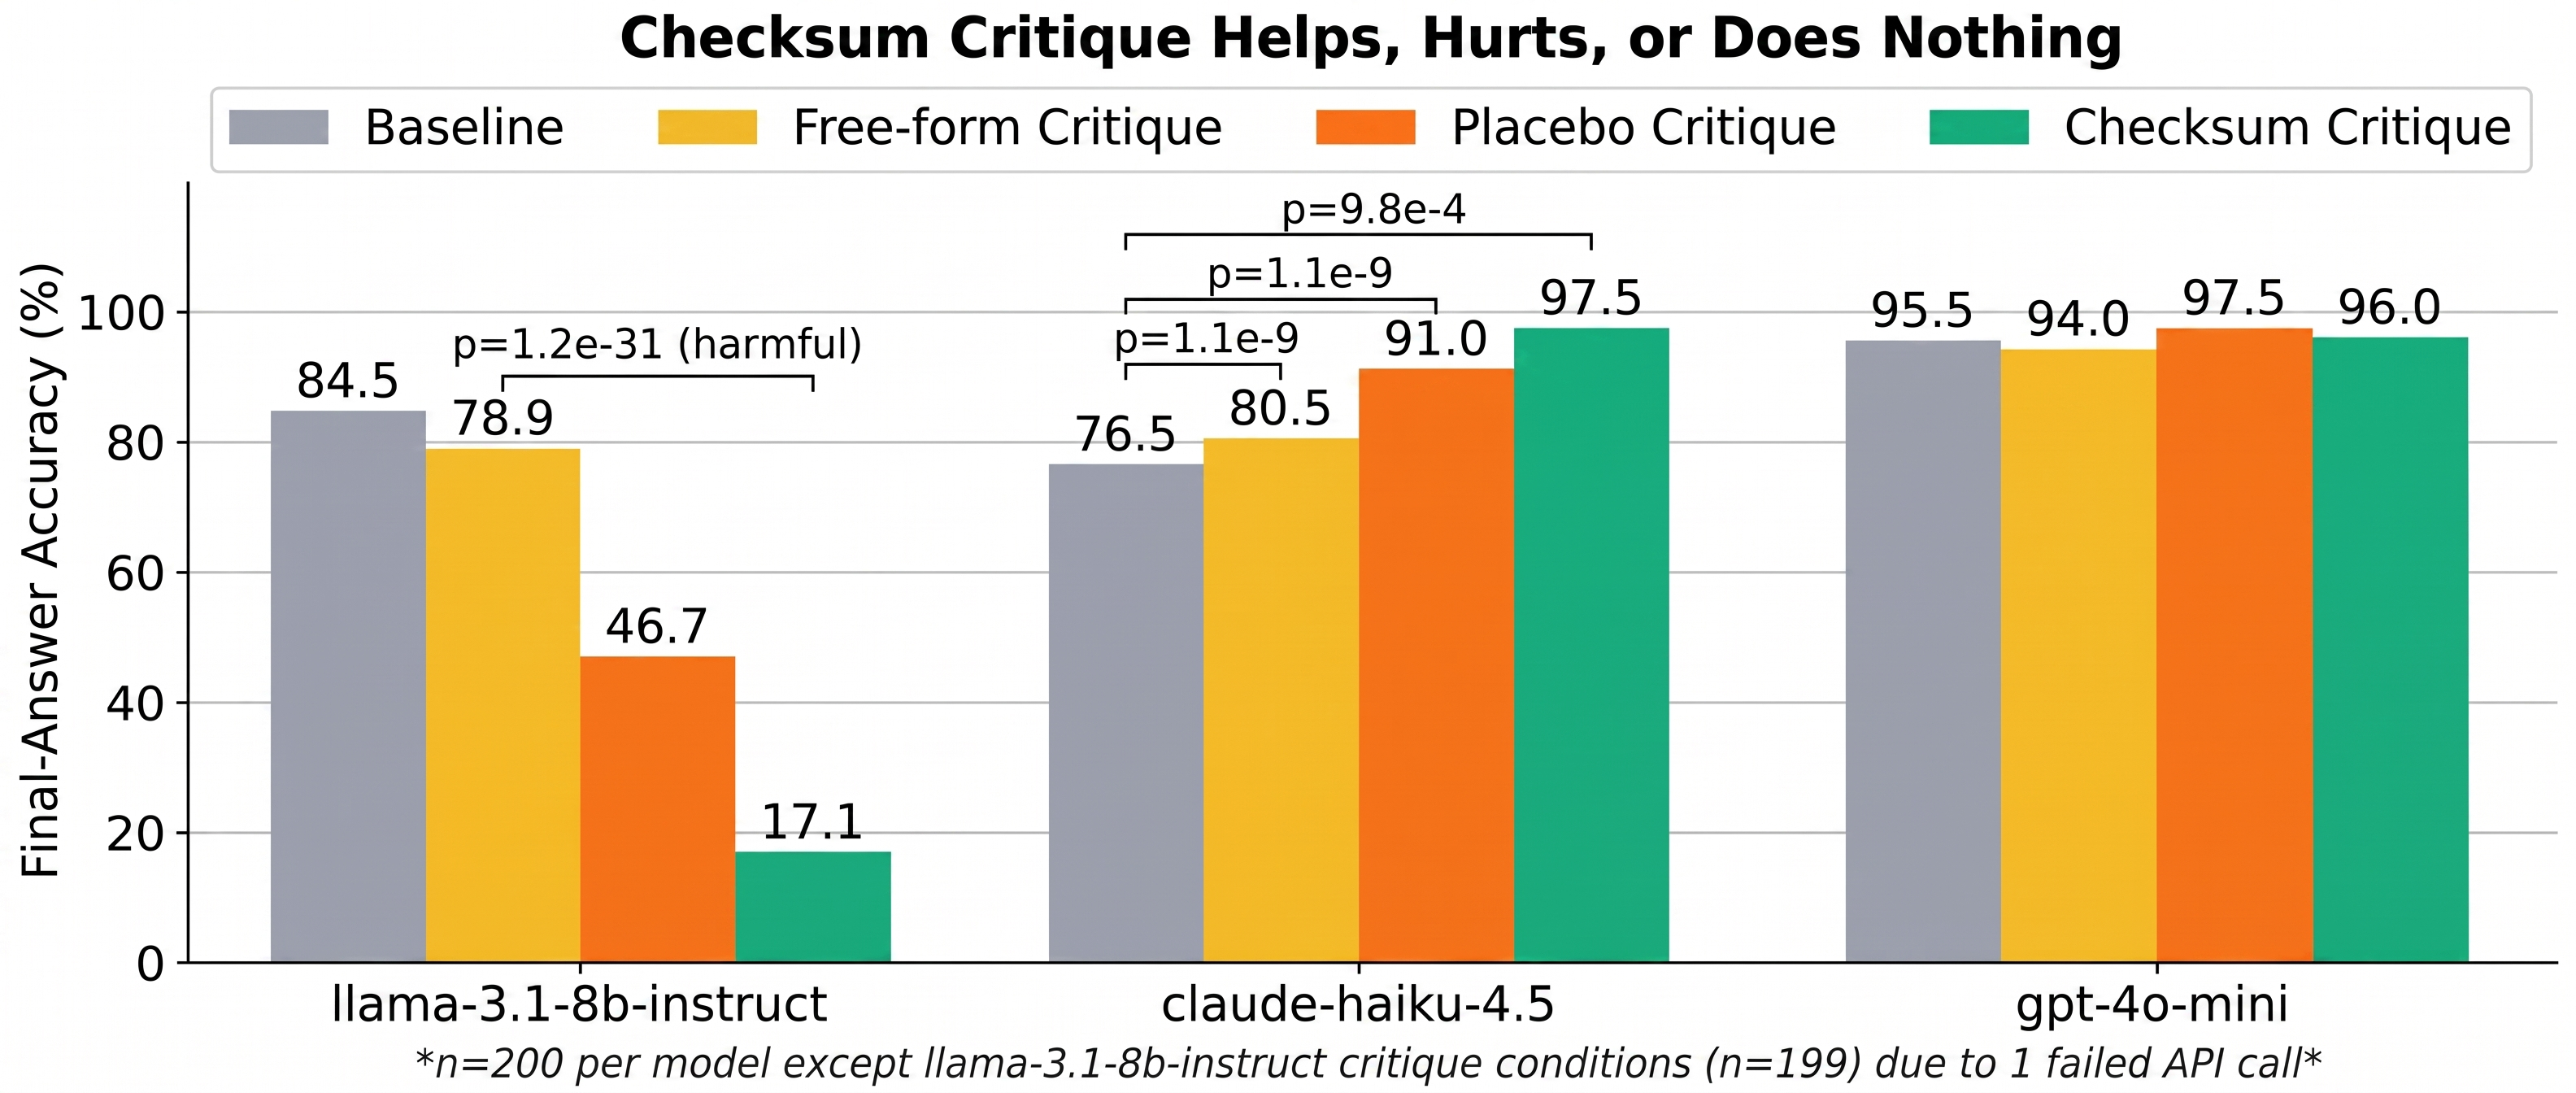
\includegraphics[width=\textwidth,height=0.45\textheight,keepaspectratio]{figures/fig2_v0.jpg}
  \caption{Final-answer accuracy by condition and model. Checksum critique produces a large gain for claude-haiku-4.5, a statistically null effect for gpt-4o-mini, and a catastrophic collapse for llama-3.1-8b-instruct, revealing a non-monotonic rather than smoothly diminishing relationship between baseline capability and checksum-critique benefit.}
  \label{fig:fig2}
\end{figure*}

\subsection{Overall Accuracy Is Capability-Stratified, Not Monotonically Diminishing}

For anthropic/claude-haiku-4.5, whose no-critique baseline accuracy is 76.5\% ($n=200$) -- leaving substantial headroom below ceiling -- self-check condition matters a great deal. Free-form critique raises accuracy modestly to 80.5\%. The matched-length placebo raises it further, to 91.0\%, confirming that generic structured deliberation carries real value independent of any specific invariant. The checksum critique raises accuracy the most, to 97.5\% overall. On the full 200-problem sample, checksum critique beats free-form critique by 17.0 percentage points (bootstrap 95\% CI [12.0, 22.0]; exact McNemar on 36 discordant pairs, $n_{01}=35$ corrected by checksum but not free-form, $n_{10}=1$ the reverse, $p=1.08\times10^{-9}$) and beats the placebo by 6.5 percentage points (bootstrap CI [3.0, 10.0]; McNemar $n_{01}=14$, $n_{10}=1$, $p=9.77\times10^{-4}$). On the checksum-detectable subset specifically ($n=64$), the checksum-vs-placebo gap is 9.375 percentage points (bootstrap CI [3.1, 17.2]).

For openai/gpt-4o-mini, the picture is a flat null result rather than a diminished-but-present effect. Baseline accuracy is already 95.5\% ($n=200$), leaving little room for any self-check condition to demonstrate an advantage: free-form critique reaches 94.0\%, the placebo reaches 97.5\%, and checksum critique reaches 96.0\%. None of these differences survive scrutiny: checksum vs. free-form is a 2.0-percentage-point gap (bootstrap CI [-2.0, 6.0], McNemar $n_{01}=11$, $n_{10}=7$, $p=0.481$), and checksum vs. placebo is a $-1.5$-percentage-point gap (bootstrap CI [-5.5, 2.0], McNemar $n_{01}=5$, $n_{10}=8$, $p=0.581$). On the checksum-detectable subset ($n=64$), the checksum-vs-placebo gap is exactly 0.0 percentage points.

For meta-llama/llama-3.1-8b-instruct, the picture inverts entirely rather than merely flattening. Baseline accuracy is 84.5\% ($n=200$) -- comparable headroom to claude-haiku-4.5's -- so a diminishing-effect-with-capability story would predict a smaller but still positive checksum benefit here. Instead, free-form critique already drops accuracy to 78.9\% ($n=199$; one of 2,592 total API calls failed for this condition), the placebo drops it further to 46.7\% ($n=199$), and checksum critique collapses it to 17.1\% ($n=199$). The checksum-vs-free-form gap is $-61.9$ percentage points (bootstrap CI [-69.5, -54.3], $n=197$ after excluding the one failed call from each side; McNemar $n_{01}=5$ cases newly correct under checksum, $n_{10}=127$ cases newly wrong, $p=1.18\times10^{-31}$), and the checksum-vs-placebo gap is $-28.9$ percentage points (bootstrap CI [-37.1, -20.8]; McNemar $n_{01}=14$, $n_{10}=71$, $p=2.43\times10^{-10}$). On the checksum-detectable subset ($n=62$ after exclusions), the checksum-vs-placebo gap is $-33.9$ percentage points (bootstrap CI [-48.4, -17.7]). Every one of these comparisons is overwhelmingly statistically significant in the harmful direction; this is not a null result obscured by noise, but a large, reliable degradation.

\begin{figure}[!htbp]
  \centering
  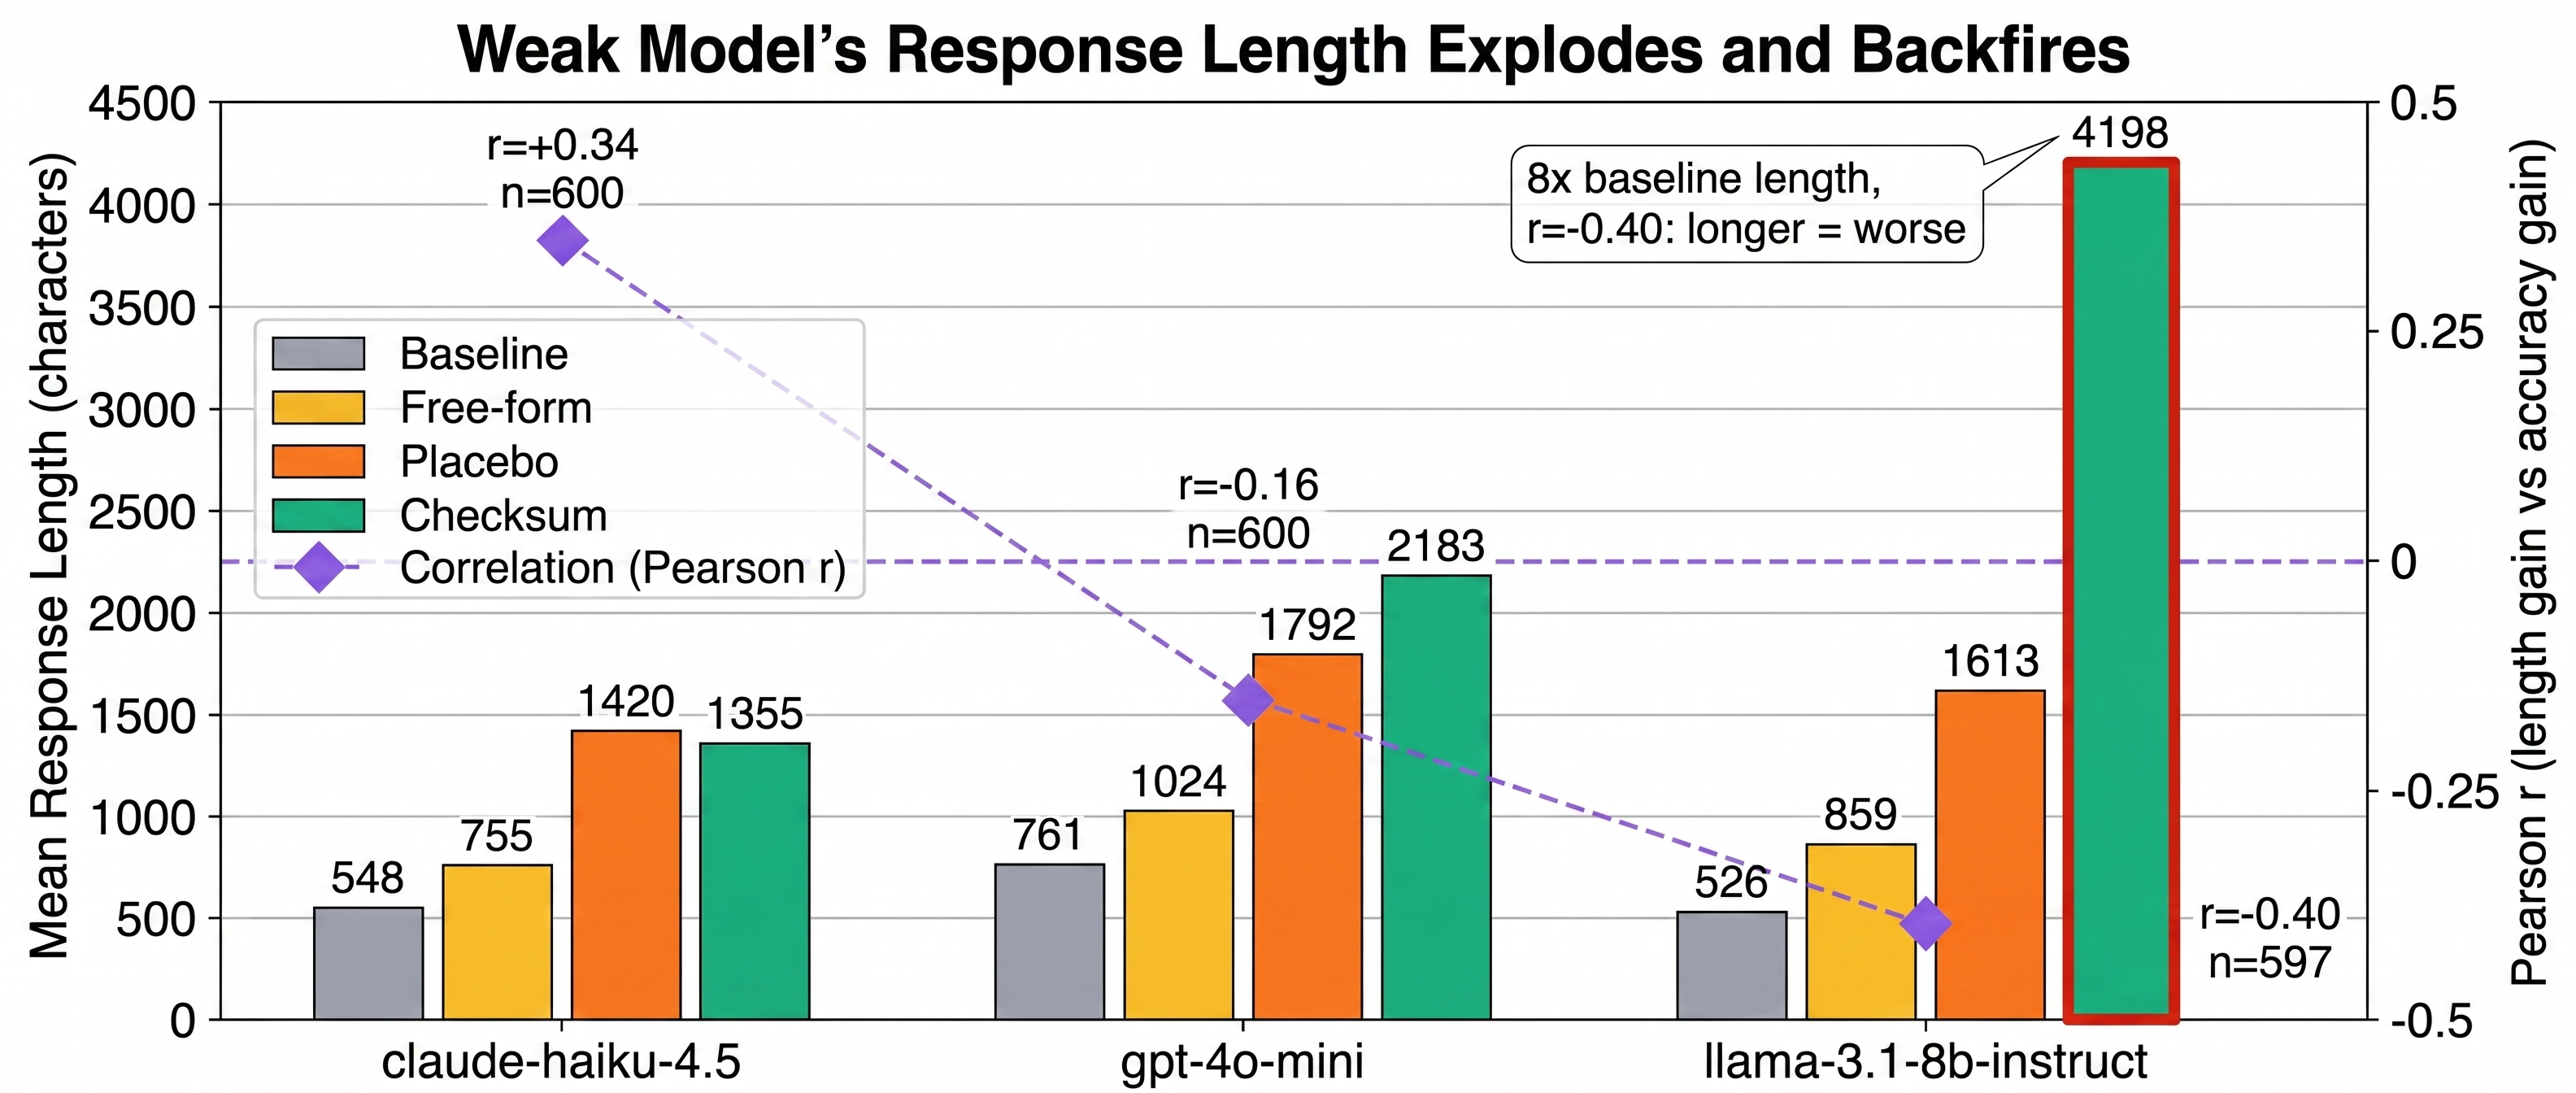
\includegraphics[width=\linewidth,height=0.4\textheight,keepaspectratio]{figures/fig3_v0.jpg}
  \caption{Mean response length by condition and model (left axis, bars) overlaid with the Pearson correlation between per-example response-length gain and accuracy gain (right axis, diamonds). llama-3.1-8b-instruct's checksum-critique responses are roughly 8x longer than its baseline, and unlike the other two models, longer checksum responses are associated with worse accuracy for this model.}
  \label{fig:fig3}
\end{figure}

\subsection{Why the Weak Model Collapses: A Bookkeeping-Overload Failure Mode}

The magnitude of llama-3.1-8b-instruct's collapse cannot be explained by the checksum condition simply flagging more errors and revising correctly-solved problems into incorrect ones: only 10 of 199 checksum-critique responses raised an explicit error flag, and correction accuracy given a genuine true-positive flag was in fact 0\% for this model in this condition (0/1 true positive corrected to the gold answer), not a source of mass corruption on its own. The dominant driver is instead visible in response length and in manual trace inspection: mean response length under checksum critique is 4,198 characters for this model, roughly 8x the 526-character no-critique baseline and more than double the placebo's 1,613-character mean, and the Pearson correlation between per-example response-length gain and per-example accuracy gain for this model is $-0.40$ ($n=597$), the strongest and most negative of the three models (claude-haiku-4.5: $+0.34$, $n=600$; gpt-4o-mini: $-0.16$, $n=600$) -- longer checksum-critique responses are associated with worse, not better, outcomes specifically for the weak model.

A representative trace illustrates the mechanism directly. On a six-step inventory word problem (starting quantity 410, three additive transactions, then a multiplicative step, correct final answer computed by the base solve), the model's checksum-critique trace correctly computes the first several digit roots, then -- partway through the checksum bookkeeping -- introduces a computation that does not correspond to any operation in the original problem (``the number of boxes is multiplied by 4''), carries this fabricated step through the remainder of its digit-root verification, and outputs a final answer that reflects neither the original problem's arithmetic nor a coherent alternative derivation. This pattern -- an unprompted extra operation appearing mid-checksum and propagating to the final answer -- recurs across the sampled traces we inspected and is consistent with the length and correlation evidence: the checksum procedure's dual demand (perform the original arithmetic correctly, and simultaneously track a second, structurally distinct digit-root computation per step) exceeds this model's capacity to keep both computations straight, and the interference corrupts the primary derivation rather than merely failing to improve it. This is qualitatively different from the free-form and placebo conditions' more modest degradations (84.5\% to 78.9\% and 46.7\% respectively), which plausibly reflect ordinary self-critique unreliability rather than induced hallucination of new problem content.

\subsection{Detection Precision, Recall, and Correction Accuracy: A Properly Powered Re-Audit}

Our previous draft's detection-metric family was reported as largely underpowered because most models rarely erred on their own baseline solve, leaving few true positives to measure against. This iteration's dedicated re-audit computes the same family of metrics with closed-form Wilson 95\% confidence intervals and an explicit underpowered-$n<20$ flag on every cell, across all three models, four conditions, and three checksum-detectability strata. The pattern confirms the accuracy-level story rather than adding a contradictory signal. For claude-haiku-4.5 under checksum critique, precision on the full sample is 1.0 (95\% CI [0.61, 1.0], 6 true positives, 0 false positives out of 200 problems) and recall is 0.128 (95\% CI [0.060, 0.252], 6 of 47 baseline-wrong problems flagged); on the checksum-invisible stratum specifically ($n=136$, by definition unreachable by a mod-9 check), recall is 0.182 (95\% CI [0.086, 0.344]), showing the checksum framing catches some errors even outside its theoretical ceiling, plausibly via the more careful step-by-step re-derivation it induces. Correction accuracy given a true-positive flag is 1.0 (6/6) for claude-haiku-4.5's checksum condition, versus 0.0 (0/1) for llama-3.1-8b-instruct's and 1.0 (1/1) for gpt-4o-mini's -- all at $n<20$ and explicitly flagged underpowered, consistent with the accuracy-level finding that llama-3.1-8b-instruct's problem is not correction given a valid flag (which happens rarely) but corruption of already-correct derivations that never gets flagged at all. gpt-4o-mini's checksum condition shows the opposite precision profile from claude-haiku-4.5's: precision is 0.053 (95\% CI [0.009, 0.246], 1 true positive against 18 false positives out of 200), i.e. this model raises many more flags than it has genuine errors to find, though this over-flagging does not translate into an accuracy cost given its near-ceiling ground truth. We report the full per-cell table, including every underpowered cell, in the evaluation artifact rather than presenting only the well-powered subset, so that a reader can judge which point estimates to trust.

\subsection{Checksum Self-Computation Reliability: Deterministic Checker Replaces Same-Model Judge}

\begin{figure}[!htbp]
  \centering
  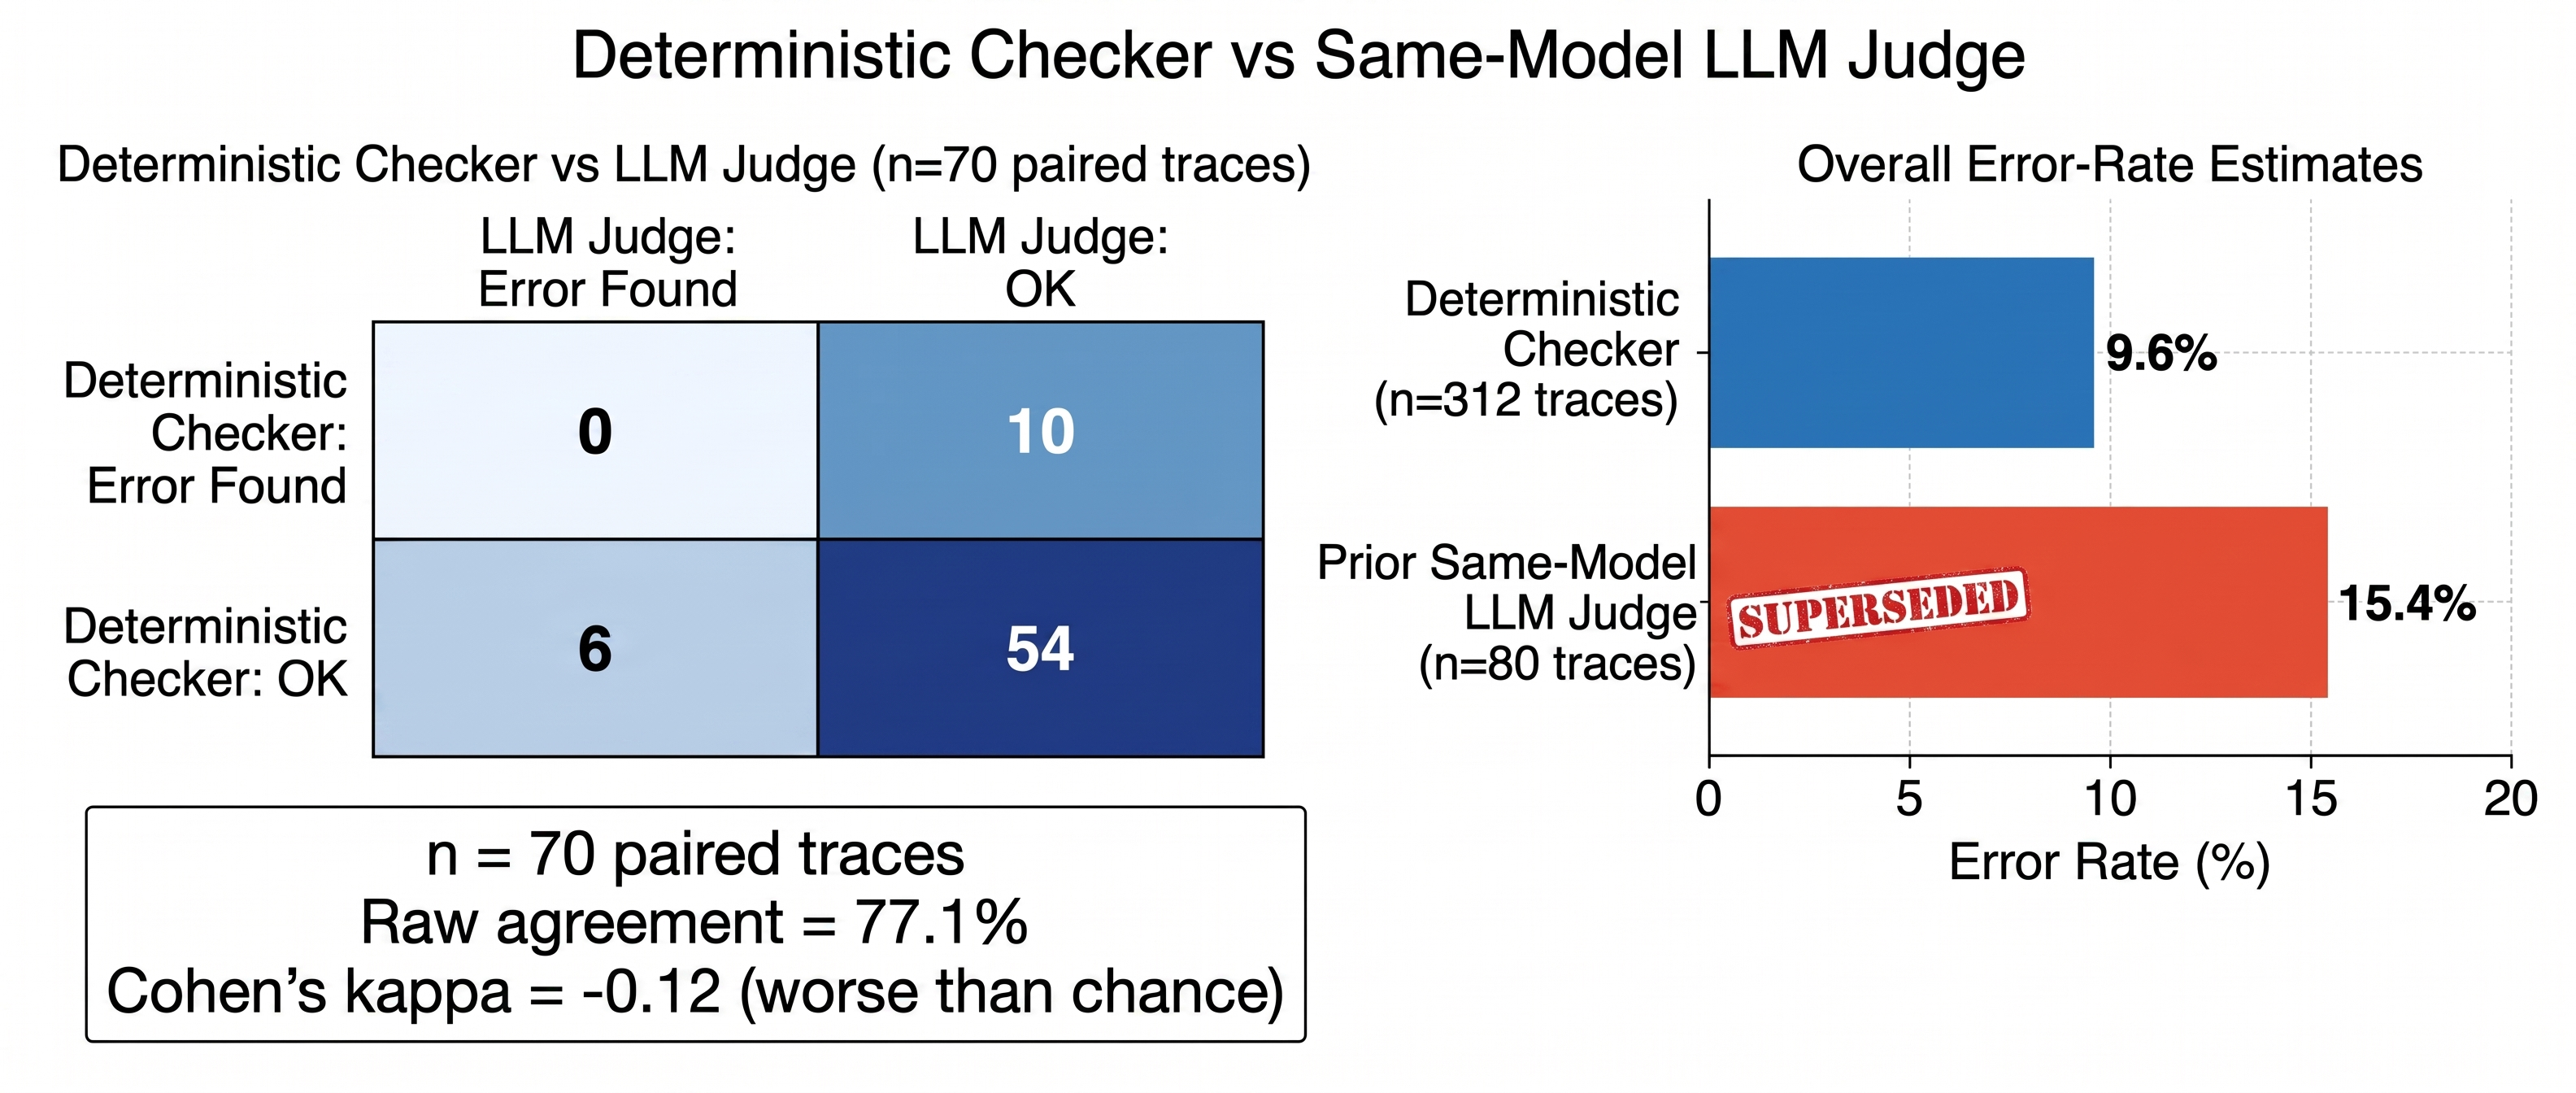
\includegraphics[width=\linewidth,height=0.4\textheight,keepaspectratio]{figures/fig4_v0.jpg}
  \caption{Agreement between the new deterministic, zero-LLM-call mod-9 checker and a freshly re-run LLM judge on the same 70 paired checksum-critique traces. Raw agreement is 77.1\%, but Cohen's kappa of $-0.12$ indicates worse-than-chance agreement once each method's own error-flagging base rate is accounted for, motivating the deterministic checker as the new primary reliability estimate (9.6\% error rate, 30/312 parseable traces) over the prior same-model-judge figure (15.4\%, 80 traces).}
  \label{fig:fig4}
\end{figure}

Our previous draft measured checksum self-computation reliability using an LLM judge (claude-haiku-4.5) that was also one of the two evaluated models -- a same-model circularity a reviewer correctly identified as a potential source of correlated bias. This iteration replaces that design with a deterministic, regex-only mod-9 digit-root checker that requires zero LLM calls: it parses every ``digit root of N'' claim across all 599 checksum-critique traces (200 claude-haiku-4.5, 199 llama-3.1-8b-instruct, 200 gpt-4o-mini), independently recomputes the true digit root via the closed-form casting-out-nines formula, and flags any trace whose claimed digit root disagrees with the recomputed one. Of 312 traces containing at least one parseable digit-root claim, 30 contain at least one arithmetic error, an overall 9.6\% error rate -- materially lower than, and now superseding, our prior same-model-judge estimate of 15.4\% (80 traces). Per-model error rates track capability in the expected direction: claude-haiku-4.5 is most reliable at the checksum sub-task (4.5\% error rate, 6/134 parseable traces), llama-3.1-8b-instruct is least reliable (12.4\%, 11/89), and gpt-4o-mini falls between (14.6\%, 13/89) -- notably, gpt-4o-mini's checksum-computation error rate is the highest of the three models even though its overall task accuracy is highest, underscoring that checksum-sub-task reliability and end-task accuracy are not the same quantity.

To validate the substitution itself, we re-ran a fresh LLM-judge pass (same prompting design as the prior draft, independently recomputing each digit-root claim before issuing a verdict) over the same 70-trace paired sample the deterministic checker evaluated, and computed Cohen's kappa between the two methods' per-trace verdicts \citep{Cohen1960}. Agreement is 77.1\% raw, but Cohen's kappa -- which corrects for chance agreement given each method's marginal error-flagging rate -- is $-0.12$, i.e. worse than chance-level agreement (confusion matrix: 0 traces where both methods agree an error is present, 6 where the checker flags an error the judge misses, 10 where the judge flags an error the checker misses, 54 where both agree the trace is clean). A negative kappa here means the LLM judge's error-flagging is essentially uncorrelated with, or anti-correlated with, ground-truth arithmetic correctness as measured by direct recomputation, which is direct evidence -- not merely a plausibility argument -- for discarding the same-model-judge design rather than treating it as a noisy-but-usable approximation. We adopt the deterministic checker's 9.6\% figure as the primary estimate going forward and treat the prior 15.4\% same-model-judge figure as superseded.

\subsection{Ruling Out Length as the Sole Driver for the Model That Benefits}

For claude-haiku-4.5, the model whose gain is causally attributable to the invariant rather than to length, response length under checksum critique (mean 1,355 characters) is close to but slightly shorter than under the placebo (mean 1,420 characters) -- a placebo-to-checksum length ratio of 1.05, i.e. the placebo is if anything slightly longer. Since checksum critique still outperforms this length-matched-or-longer placebo by 6.5 percentage points on the full sample (9.375 points on the checksum-detectable subset), the gap cannot be attributed to the checksum condition simply producing more deliberation tokens. The per-example response-length-gain-vs-accuracy-gain Pearson correlation for claude-haiku-4.5 is $+0.34$ ($n=600$, pooled across all three non-baseline conditions), positive but modest, consistent with length correlating with but not fully explaining the accuracy effect; for the two other models the same correlation is near-zero or negative (gpt-4o-mini: $-0.16$; llama-3.1-8b-instruct: $-0.40$), the opposite sign one would expect if ``more tokens helps'' were a universal mechanism. Taken together with the placebo comparison, this indicates the checksum invariant's content, not sheer verbosity, is what produces claude-haiku-4.5's gain -- and that verbosity is, if anything, actively harmful for the weak model.

\section{Discussion}

Our results substantially revise the scope of the original hypothesis, in the direction reviewer feedback pushed us toward but with a sharper conclusion than ``benefit concentrated where the model is hungry.'' With three capability tiers now evaluated -- strong (claude-haiku-4.5), mid (gpt-4o-mini), weak (llama-3.1-8b-instruct) -- the pattern is not a monotonic decline in benefit as baseline accuracy rises. It is a three-way split: a large, causally isolated positive effect for the strong model; a null effect, not a smaller positive effect, for the mid-capability model; and a large, statistically overwhelming negative effect for the weak model. We are explicit that three models is still a small panel and does not establish a general functional form (e.g. a capability threshold, a U-shaped curve, or something else) relating baseline capability to checksum-critique effect size -- we report this as a three-point pilot pattern that motivates, but does not itself confirm, a broader capability-conditioned deployment rule, and we no longer use language implying a smooth ``free lunch where the model is hungry'' trend, since the weak-model result shows headroom alone (llama-3.1-8b-instruct's 84.5\% baseline is comparable to claude-haiku-4.5's 76.5\%) does not predict the sign of the effect, let alone its magnitude.

For claude-haiku-4.5, the checksum condition beats a placebo matched for length and deterministic appearance by a significant 6.5 percentage points on the full sample and 9.375 points on the checksum-detectable subset, with the placebo's response length if anything slightly exceeding the checksum condition's. This is the strongest evidence within our design that the content of the invariant matters, not just the presence of extra structured text -- precisely the causal question a matched-effort placebo is meant to answer, and one largely absent from prior self-critique studies \citep{Madaan2023,Huang2023,Kamoi2024,Stechly2024}.

The weak-model result is, we think, the paper's most practically important finding, and one our previous two-model draft could not have surfaced. A prompt-engineering pattern that looks purely additive -- ``also do this extra mechanical check'' -- is not additive in effect when the base model cannot reliably execute two interleaved computations without interference. The manual trace evidence (Section 5) shows this is not simply ``the weak model fails to benefit''; it is ``the weak model's baseline-correct derivation gets actively corrupted by fabricated intermediate steps introduced while performing the checksum bookkeeping,'' a distinct and more concerning failure mode than the inert null result gpt-4o-mini shows. This has a direct deployment implication: any pipeline considering a mechanically-scaffolded self-critique step for cost or latency reasons (i.e. routing to a smaller model) should not assume the scaffold is safe merely because it worked well on a stronger model, and should validate the specific model-scaffold pairing rather than the scaffold in isolation.

The detection precision/recall re-audit clarifies where the strong model's remaining error lives without over-claiming what a small-$n$, single-experiment table can support: claude-haiku-4.5's checksum condition has perfect precision (no false alarms in this sample) but low recall (12.8\% overall, meaning most of its own baseline errors go unflagged), and correction given a genuine flag is perfect (6/6) though at an underpowered $n$. This is directionally consistent with our prior draft's oracle-ablation claim that correction is not the bottleneck once a flag is raised, but we no longer present that as a confirmed finding at this sample size -- the re-audit artifact's own verdict summary marks the oracle-vs-self-computed comparison as REVISED rather than confirmed, pending more true-positive cases than 200 problems at a 32\% checksum-detectable rate can supply.

The deterministic-checker replacement of our same-model LLM-judge audit is not a cosmetic methodology fix; the negative Cohen's kappa ($-0.12$) between the two methods is direct evidence that the same-model judge's verdicts were not tracking ground-truth arithmetic correctness, which retroactively undermines confidence in any conclusion our prior draft drew from that judge's 15.4\% figure beyond its role as a rough order-of-magnitude estimate. The deterministic checker's revised 9.6\% figure, and its capability-ordered per-model breakdown (4.5\% claude-haiku-4.5, 12.4\% llama-3.1-8b-instruct, 14.6\% gpt-4o-mini), is the figure we now treat as primary, and we recommend that any future self-verification-reliability audit of this kind default to a deterministic checker wherever the checked quantity (here, a closed-form arithmetic fact) admits one, rather than an LLM judge, same-model or otherwise.

We surface two further limitations candidly. First, the GSM8K-versus-procedurally-generated accuracy breakdown a reviewer specifically requested, to determine whether claude-haiku-4.5's comparatively low 76.5\% no-critique baseline reflects genuine task difficulty or a benchmark-composition artifact, remains unavailable: the experiment analyzed in this iteration used only the procedurally generated half of our benchmark (0 GSM8K-sourced items), and the run intended to exercise the full joined benchmark did not complete in time for this analysis. We mark this explicitly UNSUPPORTED/pending rather than approximating it, and flag it as the single highest-priority item for the next iteration, since the dataset needed to answer it already exists and is fully verified. Second, our benchmark's procedurally generated problems draw numeric ranges and chain lengths (up to 6 steps, operands up to several hundred) that are somewhat more demanding than typical GSM8K items, which plausibly contributes to baseline accuracies below commonly reported GSM8K figures independent of any GSM8K-specific effect; we cannot yet decompose these two contributions without the pending GSM8K-split run.

\section{Conclusion}

Replacing an open-ended ``check your work'' instruction with an explicit, mechanically-computed casting-out-nines checksum does not act as a uniform reliability upgrade. Across three models spanning strong, mid, and weak baseline capability, we find a genuine, causally isolated, statistically significant improvement for the strong model (claude-haiku-4.5: 76.5\% to 97.5\% overall accuracy, beating a length-matched placebo by 6.5 to 9.375 percentage points depending on subset), no measurable effect for the mid-capability model already near ceiling (gpt-4o-mini: 95.5\% baseline, every pairwise condition comparison statistically indistinguishable), and a large, statistically overwhelming degradation for the weak model (llama-3.1-8b-instruct: 84.5\% to 17.1\%, driven by the checksum procedure's bookkeeping load inducing hallucinated computation steps that corrupt an otherwise-correct derivation). This three-way, non-monotonic pattern is the central empirical correction this iteration makes to our own prior two-model draft, and it argues against treating ``give the model a mechanically-defined invariant instead of a vague instruction'' as a general-purpose self-critique fix; the fix's value is conditional on the underlying model's capacity to execute the added mechanical procedure without interference, not merely on its having room to improve. A deterministic, LLM-free re-audit of checksum self-computation reliability supersedes our earlier same-model LLM-judge estimate (15.4\%, itself shown here to disagree with the deterministic ground truth at worse-than-chance levels, Cohen's kappa$=-0.12$) with a lower, more trustworthy figure (9.6\%, 30/312 parseable traces), and a properly powered precision/recall/F1 re-audit replaces the underpowered proxy metric our previous draft candidly flagged as a design limitation.

Future work should prioritize, in order: (1) completing the pending run that joins the four critique conditions against the full GSM8K-plus-synthetic benchmark, including its 1,535 labeled error-injection variants, to obtain the GSM8K-vs-synthetic baseline decomposition and the ground-truth-labeled detection precision/recall analysis this iteration still cannot fully deliver; (2) extending the model panel beyond three points, particularly with models between llama-3.1-8b-instruct's and gpt-4o-mini's capability level, to determine whether the observed strong-null-catastrophic pattern reflects a sharp capability threshold or a smoother underlying relationship we lack the resolution to distinguish; and (3) directly instrumenting why the checksum procedure specifically induces hallucinated computation steps in weaker models -- for example, by testing whether providing the checksum bookkeeping in a separate, sequential turn rather than an interleaved single-turn instruction avoids the interference we document here.

\appendix
\section{Verbatim Critique Condition Prompts}

All four solve-time conditions share the identical base solve instruction: ``Solve this problem step by step and give the final numeric answer as `Answer: \texttt{<n>}'.\\ \\ Problem: \{problem\}''. Each critique condition appends the following text to that base instruction.

\textbf{Free-form critique:} ``Then check your work above for mistakes. If you find an error, correct it and give a final revised answer as `Answer: \texttt{<n>}'.''

\textbf{Placebo critique:} ``Then, for EACH arithmetic sub-step above, restate the two operand values and the result value, spell out each of their digits one by one in words (e.g. `four, two, one'), count how many digits each number has, and state whether the result has more, fewer, or the same number of digits as the larger operand. Show this digit-listing review explicitly for every step (this is a formatting/presentation review, not a mathematical re-check, and finding more/fewer/same digits does NOT by itself indicate an error). If, separately, you notice an actual arithmetic error while doing this, correct it and give a final revised answer as `Answer: \texttt{<n>}'.''

\textbf{Checksum critique:} ``Then, for EACH arithmetic sub-step above, compute the digit root (repeatedly sum the digits of a number until one digit remains) of each operand and of the result, and verify the operands' digit-root relationship matches the result's digit root under mod-9 arithmetic (this is the `casting out nines' checksum). Show each step's digit-root check explicitly, ending each check with either CHECKSUM\_OK or CHECKSUM\_MISMATCH. Only revise a step if its digit roots are inconsistent. Give a final revised answer as `Answer: \texttt{<n>}'.''

\textbf{Oracle detection-isolation ablation} (checksum-detectable subset only): base solve instruction plus ``A checker has flagged that your step `\{step\_desc\}' has a casting-out-nines checksum mismatch: digit\_root(\{a\}) \{op\} digit\_root(\{b\}) should equal digit\_root(\{correct\_result\}) under mod-9 arithmetic, but your computed result of \{wrong\_result\} does not satisfy this. Fix this step and give the final revised answer as `Answer: \texttt{<n>}'.''

All conditions were sampled at temperature 0.0 with a 2,500-token generation budget via OpenRouter.

\bibliographystyle{plainnat}
\bibliography{references}

\end{document}
